\chapter{Spectral and Matrix-Analytic Arguments}
\setcounter{section}{-1}   % sections start at 8.0 (see main.tex comment)
\label{ch:spec}

\begin{objectives}
\item Recognize when a system's state is a matrix in disguise: transitions, affinities, recursions, Gram matrices.
\item Prove the ladder Rayleigh $\to$ Perron--Frobenius $\to$ Neumann $\to$ interlacing $\to$ low rank/projection.
\item Turn spectral facts into guarantees: rates, invertibility, subspace optimality, distance preservation.
\item Name the matrix, localize the spectrum, exploit the gap or the rank.
\end{objectives}

Spectral and matrix-analytic arguments replace a sprawling object --- a graph,
a recursion, a point set --- with the few numbers that govern its behavior
under repetition: eigenvalues, singular values, spectral radii, eigengaps.
Find the linear map inside the artifact --- a random walk applies a
transition matrix, a smoothness objective is a quadratic form --- then read
the answer off the spectrum: does iteration converge, how fast, and which
subspace carries the object?

In the SIGMOD'26 corpus, 13 papers are tagged with this machinery, pairing it
with graph analytics (spectral clustering of multi-relational graphs, exact
SimRank-style similarity), high-dimensional vector search (subspace
projections and collision counting), and fairness pre-processing through
latent attributes --- plus, a reminder that the tool respects no domain
boundaries, the space utilization of B-tree leaves under batched
insertions. The chapter builds the ladder (Section~\ref{sec:spec-tool}),
dissects four exemplars (Sections~\ref{sec:spec-btree}--\ref{sec:spec-pjsim}), and closes with advanced sketches and further reading
(Section~\ref{sec:spec-advanced}).

\section{The tool: spectral and matrix arguments}
\label{sec:spec-tool}

The problem class is uniform: a square matrix $A$ sits inside the system as
the transition applied by one update step, the quadratic form being
minimized, or the structure behind a vectorized equation; the deliverable
--- limits, solvability, subspaces, distortion --- is decided by where the
eigenvalues of $A$ sit (Figure~\ref{fig:spec-spectrum}).

\begin{remarkbox}[Notation]
$A \in \mathbb{R}^{d \times d}$; for symmetric $A$, eigenvalues $\lambda_1 \ge
\dots \ge \lambda_d$. Operator norm $\|A\|_2$, Frobenius norm $\|A\|_F$,
spectral radius $\rho(A) = \max_i |\lambda_i(A)|$; $A \ge 0$ is entrywise.
$G[A]$: an edge $i \to j$ iff $A_{ij} \ne 0$; $A$ is \emph{irreducible} if
$G[A]$ is strongly connected, \emph{Metzler} if its off-diagonal entries are
nonnegative. $A \otimes B$ is the Kronecker product,
$A \oplus B = (A \otimes I) + (I \otimes B)$ the Kronecker sum,
$\operatorname{Vec}(\cdot)$ stacks columns.
\end{remarkbox}

\subsection{The basic ladder}
\label{sec:spec-ladder}

Eigenvalues are the extreme values of a scalar function of the direction.

\begin{theorem}[Rayleigh quotient]\label{thm:spec-rayleigh}
Let $A = A^{\top} \in \mathbb{R}^{d \times d}$ have eigenvalues $\lambda_1 \ge
\dots \ge \lambda_d$ and orthonormal eigenvectors $v_1,\dots,v_d$. For the
Rayleigh quotient $R(x) = \frac{x^{\top}\!A x}{x^{\top}x}$, $x \ne 0$,
\[
\lambda_1 = \max_{x \ne 0} R(x),
\qquad \lambda_d = \min_{x \ne 0} R(x). \eopm
\]
\end{theorem}

\begin{proof}
$R(x) = \sum_i \lambda_i c_i^2 / \sum_i c_i^2$ for $x = \sum_i c_i v_i$ is a
convex combination of the eigenvalues --- at most $\lambda_1$, at least
$\lambda_d$, with equality at $x = v_1$, $v_d$.
\end{proof}

Most matrices in database papers are not symmetric but \emph{nonnegative} ---
counts, probabilities, affinities --- and there a structure theorem applies
\citep{spectral-matrix-bg1,spectral-matrix-bg5}:

\begin{theorem}[Perron--Frobenius]\label{thm:spec-pf}
Let $A \ge 0$ be irreducible. Then $\rho(A) > 0$ is an eigenvalue of $A$; it
is simple; it admits entrywise positive left and right eigenvectors; and
every other eigenvalue $\lambda \ne \rho(A)$ satisfies
$\operatorname{Re}(\lambda) < \rho(A)$. \eop
\end{theorem}

\begin{proof}[Proof sketch]
Irreducibility makes $A$ eventually map the nonnegative cone into its
interior, so $x \mapsto Ax/\|Ax\|_1$ has an interior simplex fixed point ---
a positive eigenvector for $\rho(A)$; a rank-one positive perturbation shows
the eigenvalue is simple and dominates in real part
\citep{spectral-matrix-bg1}.
\end{proof}

The B-tree exemplar (\citep{sigmod26-038}; Section~\ref{sec:spec-btree}) has
a negative diagonal instead --- a shift by $cI$ fixes that:

\begin{corollary}[Metzler variant, Lemma of \citep{sigmod26-038}, notation
cleaned]\label{cor:spec-metzler}
Let $A$ be an irreducible Metzler matrix admitting an entrywise positive $w$
with $w^{\top}\!A = r\,w^{\top}$, $r > 0$. Then $r$ is a simple eigenvalue
with a positive right eigenvector, and every other eigenvalue $\lambda$
satisfies $\operatorname{Re}(\lambda) < r$. \eop
\end{corollary}

\begin{proof}
$B = A + cI \ge 0$ (with $c = \max_i |A_{ii}|$) is irreducible, and
$w^{\top}\!B = (r+c)\,w^{\top}$ is a positive left eigenvector, which
Perron--Frobenius (Theorem~\ref{thm:spec-pf}) assigns to $\rho(B) = r+c$:
simple, positive right eigenvector, dominant in real part. Since
$\sigma(B) = \sigma(A) + c$, the claims transfer.
\end{proof}

The second rung turns spectral location into a rate: a spectrum strictly
inside the unit disk makes the inverse of $I - A$ a geometric series
\citep{spectral-matrix-bg1}.

\begin{theorem}[Neumann series with truncation rate]\label{thm:spec-neumann}
Let $\rho(A) < 1$. Then $I - A$ is invertible with $(I-A)^{-1} = \sum_{k \ge 0}
A^k$, and for any submultiplicative norm with $\|A\| \le q < 1$ the partial
sum $S_L = \sum_{k=0}^{L} A^k$ obeys
\[
\bigl\|(I-A)^{-1} - S_L\bigr\| \;\le\; \frac{q^{L+1}}{1-q}. \eopm
\]
\end{theorem}

\begin{proof}
$(I-A)S_L = I - A^{L+1}$ and $\|A^{L+1}\| \le q^{L+1} \to 0$; the tail is the
geometric series $\sum_{k > L} q^k$.
\end{proof}

The third rung governs \emph{subspaces}: compressing a symmetric matrix to a
smaller orthonormal basis sandwiches the eigenvalues between those of the
original, making ``which eigenvectors do I keep'' a well-posed optimization
\citep{spectral-matrix-bg1,spectral-matrix-bg2}.

\begin{theorem}[Courant--Fischer and Poincar\'e separation]\label{thm:spec-interlace}
(Courant--Fischer) For symmetric $A$ with eigenvalues $\lambda_1 \ge \dots \ge
\lambda_d$,
\[
\lambda_k(A) \;=\; \min_{\substack{V \subseteq \mathbb{R}^d\\ \dim V = d-k+1}}
\;\max_{0 \ne x \in V} R(x)
\;=\; \max_{\substack{V \subseteq \mathbb{R}^d\\ \dim V = k}}
\;\min_{0 \ne x \in V} R(x).
\]
(Poincar\'e separation) If $B \in \mathbb{R}^{d \times s}$ has orthonormal
columns and $\mu_1 \ge \dots \ge \mu_s$ are the eigenvalues of
$B^{\top}\!A B$, then $\lambda_i(A) \ge \mu_i \ge \lambda_{d-s+i}(A)$,
$i = 1,\dots,s$. \eop
\end{theorem}

\begin{proof}[Proof sketch]
Courant--Fischer: the max--min is attained on the top $k$ eigenvectors' span,
and no $k$-dimensional subspace guarantees more (exchange argument).
Poincar\'e: $B^{\top}\!A B$ is $R$ restricted to $\operatorname{span}(B)$;
Courant--Fischer inside that subfamily sandwiches each $\mu_i$. Full proof
in Section~\ref{sec:spec-appendix}.
\end{proof}

The fourth rung certifies throwing information away: the residual of a
truncated decomposition is governed exactly by the first discarded singular
values \citep{spectral-matrix-bg1,spectral-matrix-bg3,spectral-matrix-bg4}.

\begin{theorem}[Eckart--Young--Mirsky]\label{thm:spec-eym}
Let $A \in \mathbb{R}^{m \times n}$ have singular values $\sigma_1 \ge
\sigma_2 \ge \dots \ge 0$ and singular vectors $u_i, v_i$. Then for every $B$
of rank at most $r$,
\[
\|A - B\|_2 \;\ge\; \sigma_{r+1},
\qquad
\|A - B\|_F \;\ge\; \Bigl(\textstyle\sum_{i > r} \sigma_i^2\Bigr)^{1/2},
\]
and the truncated SVD $A_r = \sum_{i \le r} \sigma_i u_i v_i^{\top}$ attains
both bounds. \eop
\end{theorem}

\begin{proof}[Proof sketch]
$\|A - A_r\| = \sigma_{r+1}$ by inspection of the tail; for the lower bound,
the span of the top $r+1$ right singular vectors meets the kernel of any
rank-$\le r$ $B$, and on a unit $x$ there $\|(A-B)x\|_2 = \|Ax\|_2 \ge
\sigma_{r+1}$. Full proof (both norms) in Section~\ref{sec:spec-appendix}.
\end{proof}

The last rung makes distances cheap: a random low-dimensional projection is
an approximate isometry, with dimension set by accuracy and the number of
events to survive \citep{spectral-matrix-bg3,spectral-matrix-bg4}.

\begin{theorem}[Distributional Johnson--Lindenstrauss]\label{thm:spec-jl}
Let $A \in \mathbb{R}^{d \times D}$ consist of the first $d$ rows of a
uniformly random orthogonal $D \times D$ matrix. Then for every fixed $x \in
\mathbb{R}^D$, $\mathbb{E}\|Ax\|_2^2 = \tfrac{d}{D}\|x\|_2^2$, and for
$\varepsilon, \beta \in (0,1)$ with $d \ge C\,\varepsilon^{-2}\ln(1/\beta)$,
\[
\Pr\Bigl[\;\Bigl|\|Ax\|_2^2 - \tfrac{d}{D}\|x\|_2^2\Bigr| >
\varepsilon\,\tfrac{d}{D}\|x\|_2^2\Bigr] \;\le\; \beta. \eopm
\]
\end{theorem}

\begin{proof}[Proof sketch]
A random orthogonal map takes $x/\|x\|$ to a uniformly random direction, so
$\|Ax\|_2^2/\|x\|_2^2$ is distributed like the squared length of the first $d$
coordinates of a uniform point on the sphere --- approximately $\chi^2_d/d$,
whose concentration gives failure probability $2e^{-\Theta(\varepsilon^2 d)}$;
full proof in Section~\ref{sec:spec-appendix}.
\end{proof}

\begin{widefigure}[t]
\centering
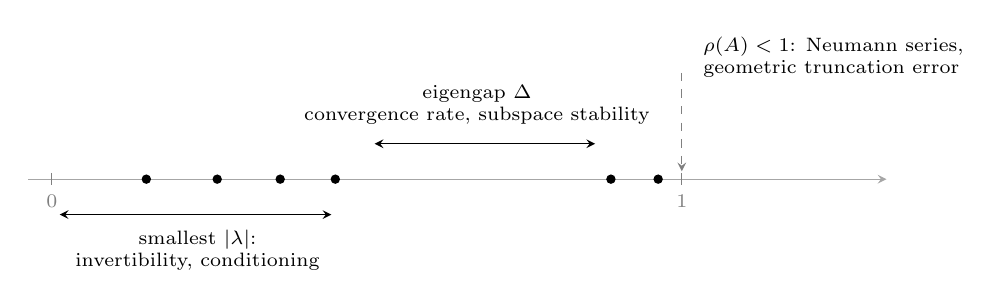
\begin{tikzpicture}[>=stealth]
  \draw[->, gray!70] (-0.3,0) -- (10.6,0);
  \draw[gray] (0,0.08) -- (0,-0.08) node[below, font=\scriptsize, gray] {$0$};
  \draw[gray] (8,0.08) -- (8,-0.08) node[below, font=\scriptsize, gray] {$1$};
  \foreach \x in {1.2, 2.1, 2.9, 3.6, 7.1, 7.7} \fill (\x,0) circle (1.7pt);
  \draw[<->] (4.1,0.45) -- (6.9,0.45);
  \node[font=\scriptsize, align=center] at (5.4,0.95)
    {eigengap $\Delta$\\ convergence rate, subspace stability};
  \draw[<->] (0.1,-0.45) -- (3.55,-0.45);
  \node[font=\scriptsize, align=center] at (1.85,-0.9)
    {smallest $|\lambda|$:\\ invertibility, conditioning};
  \draw[->, gray, dashed] (8,1.35) -- (8,0.1);
  \node[font=\scriptsize, align=left, anchor=west] at (8.15,1.55)
    {$\rho(A) < 1$: Neumann series,\\ geometric truncation error};
\end{tikzpicture}
\caption{Reading a spectrum: distance from $0$ certifies invertibility; a
spectral radius below $1$ licenses a Neumann expansion; a large eigengap
$\Delta$ fixes rates and subspace stability.}
\label{fig:spec-spectrum}
\end{widefigure}

\subsection{How to choose the matrix lens}
\label{sec:spec-choose}

The selection is mechanical. \emph{What are the entries?} Transition counts
or probabilities point at Perron--Frobenius; an optimized quadratic form at
Rayleigh/Courant--Fischer; a huge structured linear system at spectrum
localization plus Neumann; fast-decaying singular values at low-rank
truncation; expensive distances at random projection. \emph{What property is
needed?} Existence needs the spectrum clear of zero; a rate needs a radius
or gap; a subspace recommendation needs interlacing; $(1\pm\varepsilon)$
distances need the JL dimension. \emph{Not symmetric?} Perron--Frobenius, Schur triangularization, or singular values.

\begin{reachbox}{When to Reach for Spectral Arguments}
Reach whenever the object is governed by repetition --- random walks,
recursive similarity, iterative updates, insertion sequences --- or a
combinatorial objective (clustering, subspace selection) hides a quadratic
form. Then run the recipe:
\begin{enumerate}
\item \textbf{Name the matrix}: write down the linear map that one step (one
  batch, one iteration, one hop) applies, and what its entries mean.
\item \textbf{Check the structure}: nonnegative and irreducible $\to$
  Perron--Frobenius (Metzler variant if the diagonal is negative); symmetric
  $\to$ Rayleigh/interlacing; contraction ($\rho < 1$, or eigenvalues in
  $[0,1]$) $\to$ Neumann; fast singular-value decay $\to$ truncated SVD;
  expensive distances $\to$ random projection.
\item \textbf{Localize the spectrum}: row sums, Gershgorin discs,
  stochasticity, or the Kronecker-sum identity $\lambda(A \oplus B) =
  \lambda_i(A) + \lambda_j(B)$ --- place the spectrum relative to $0$ and
  $1$ and bound the dominant gap.
\item \textbf{Convert to the guarantee}: radius $\to$ geometric rate; gap
  $\to$ subspace stability and stopping rule; singular tail $\to$ rank-$r$
  error; projection dimension $\Theta(\varepsilon^{-2}\log(
  \text{events}/\delta))$, union-bounded over all points preserved.
\end{enumerate}
\end{reachbox}

\section{B-tree fragmentation under batched insertions}
\label{sec:spec-btree}

The exemplar is a PODS'26 paper on the space utilization of B-trees
\citep{sigmod26-038}\pods. When a B-tree leaf fills up and splits, the new
leaves start out on average half empty --- underfull leaves mean more cache
misses and rebalancing downstream. Yao's seminal result shows that even
splitting against uniformly random single-key insertions achieves about
$69\%$ space utilization. Many applications, however, insert in
\emph{batches} --- runs of consecutive keys at one position --- a regime
Yao's fringe analysis does not cover. The paper generalizes fringe analysis
to batched workloads: even splitting provably keeps working for many of
them, and simple alternatives cover the remaining regimes.

\paragraph{Problem.}
A B-tree stores keys in leaves (blocks) of capacity $B$. The workload is
random batched insertions: each batch is $r$ consecutive keys inserted at a
uniformly random position, and a \emph{split strategy} decides how an
overflowing block is partitioned. \emph{Fringe analysis} tracks the
histogram of block occupancies --- after $n$ keys, the vector $x^n =
(x^n_k)$ counts blocks of each size $k$ --- and asks for the \emph{expected
final fullness}, the limit of average block size normalized by $B$.

\paragraph{Guarantee.}

\begin{theorem}[Deferred even split fullness, Lemma of \citep{sigmod26-038},
notation cleaned]\label{thm:spec-btree-fullness}
Let $B$ and $i$ be positive integers with batch size $r \in \bigl(B/(2i),\,
B/(2i-1)\bigr]$. Under the deferred even split strategy (a block is split
evenly only when it overflows), the expected final fullness is
\[
\frac{2ir}{B}\,\bigl(H_{2i} - H_i\bigr),
\qquad
H_k = 1 + \tfrac{1}{2} + \dots + \tfrac{1}{k}. \eopm
\]
\end{theorem}

\sidenote{Sanity checks: $r = B$ ($i = 1$) gives fullness $1$; $r = 1$ ($i
\approx B/2$) gives $\approx \ln 2 \approx 0.693$ --- exactly Yao's
classical $69\%$.}

\paragraph{How spectral analysis is applied.}
The named object is the expectation vector $z_n = \mathbb{E}[x^n]$. Since one
batch is linear on the histogram, $z_n$ satisfies an exact \emph{matrix
recurrence}
\[
z_{n+r} \;=\; \Bigl(I + \tfrac{1}{n} A(B,r)\Bigr)\, z_n,
\]
where the $k$-th column of $A(B,r)$ records the net histogram change when a
batch of $r$ keys hits a block of size $k$. $A(B,r)$ is Metzler, and on the
class $S$ of reachable block sizes (a cycle modulo $r$ in the pattern graph)
the principal submatrix $A(B,r)_S$ is irreducible: $w_k = k$ satisfies
$w^{\top}A(B,r)_S = r\,w^{\top}$ (a batch always adds $r$ keys), so
Corollary~\ref{cor:spec-metzler} makes $r$ a simple dominant eigenvalue
with positive eigenvector. Convergence of the recurrence is the workhorse.

\begin{theorem}[Convergence of the matrix recurrence, Theorem of
\citep{sigmod26-038}, notation cleaned]\label{thm:spec-btree-recurrence}
Let $v_{n+r} = \bigl(I + \tfrac{1}{n}A\bigr) v_n$ for $n \ge n_0$, where $r \in
\sigma(A)$ is a simple positive eigenvalue dominating in real part. Then
\[
\lim_{m \to \infty} \frac{v_{n_0 + mr}}{n_0 + mr}
\;=\; P_r^A\Bigl(\frac{v_{n_0}}{n_0}\Bigr),
\]
where $P_r^A$ is the spectral projection onto the generalized eigenspace of
$r$. \eop
\end{theorem}

\begin{proof}[Proof sketch]
Iterating, $v_{n_0+mr} = \bigl(\prod_{k=0}^{m-1} (I +
\frac{1}{n_0+kr}A)\bigr) v_{n_0}$. In Jordan form the mode for $\lambda$
with block size $d$ evolves as scalars $(1 + \lambda/(n_0+kr))$ times a
nilpotent part; the product bound (Lemma~\ref{lem:spec-btree-prod}) shows
the dominant mode grows like $m$, every other like $o(m)$ or $(\ln m)^d$ ---
only the dominant spectral projection survives after division by $m$.
\end{proof}

\begin{lemma}[Scalar product bound, Lemma of \citep{sigmod26-038}, notation
cleaned]\label{lem:spec-btree-prod}
For positive integers $n_0, r$ and $\lambda \in \mathbb{C}$,
\[
\Bigl|\prod_{k=0}^{m-1} \Bigl(1 + \frac{\lambda}{n_0 + kr}\Bigr)\Bigr|
\;\le\; m^{\operatorname{Re}(\lambda)/r}\cdot \alpha_{\lambda, n_0, r},
\]
for a constant $\alpha_{\lambda,n_0,r}$ independent of $m$. \eop
\end{lemma}

\begin{proof}[Proof sketch]
Pointwise $|1+t| \le \exp\!\bigl(\operatorname{Re}(t) + \tfrac{1}{2}|t|^2
\bigr)$; summing over $k$, $\sum_k \operatorname{Re}\bigl(\lambda/(n_0+kr)
\bigr) = \frac{\operatorname{Re}(\lambda)}{r}\ln m + O(1)$ (integral
comparison) and $\sum_k |\lambda|^2/(n_0+kr)^2 = O(1)$. Full proof in
Section~\ref{sec:spec-appendix}.
\end{proof}

The last step is pure \emph{eigenvector arithmetic}. By
Theorem~\ref{thm:spec-btree-recurrence} the normalized histogram converges
into the eigenspace of $r$, and a lemma of the paper pins the limit of the
expected average block size to $\langle u, w\rangle_S / \langle u,
1\rangle_S$ for \emph{any} eigenvector $u$ --- a weighted average over any
partition of $S$, hence at least the minimum class ratio. Three partitions
give three bounds, each favorable in its regime ($r < 0.0058B$, $r < 0.21B$,
$0.21B \le r < 0.5B$), and the eigenvector recurrence $u_k =
\frac{k-r}{k+r}\,u_{k-r}$ (Lemma of the paper) yields the $H_{2i} - H_i$ of
Theorem~\ref{thm:spec-btree-fullness}; the knob $r/B$ selects even, uneven,
or the paper's TargetSplit for long batches.

\paragraph{What it buys.}
The storage engine gets provable utilization numbers per batch-size regime
--- even splitting near-optimal for small $r$, uneven splits above $7/12$ fullness, TargetSplit exact for long batches --- all from one pattern:
recurrence, dominant eigenvalue, product bound, eigenvector arithmetic.

\section{Clustering multi-relational graphs by Dirichlet energy}
\label{sec:spec-mrg}

The exemplar is a SIGMOD'26 paper on clustering large multi-relational graphs
\citep{sigmod26-303}. Multi-relational graphs (MRGs) model objects connected
by many types of interaction at once; partitioning their $N$ nodes into $K$
clusters is a fundamental analytics task. Existing solutions either fuse
the heterogeneous relations so crudely that result quality collapses, or
lean on heavyweight deep models that cannot scale to billions of edges. The
paper proposes DEMM and its scalable sibling DEMM+: first derive node
feature vectors by minimizing a \emph{multi-relational Dirichlet energy}
(a smoothness functional over all relations), then cluster by minimizing
Dirichlet energy over the resulting affinity graph --- DEMM+ never
materializes the dense $N \times N$ matrix and runs in linear time. The
spectral content is threefold: a Neumann series computes the smoothed
embedding, Courant--Fischer-type bounds certify the series is legal, and a
Sinkhorn balancing makes the final step equivalent to plain $k$-means.

\paragraph{Problem.}
Let $G$ be an MRG with $N$ nodes and $R$ relation types; relation $r$ induces
a symmetric normalized affinity $S^{(r)}$, and $S = \sum_{r=1}^{R} \omega_r
S^{(r)}$ with $\sum_r \omega_r = 1$ is the fused affinity. The clustering
objective is a normalized-cut-type quantity over node-cluster incidence
matrices $Y$, equivalent to trace maximization $\max_Y
\operatorname{trace}(Y^{\top}\!SY)$ under combinatorial constraints ---
NP-hard, and it needs the dense matrix $S$. Stage one replaces hard
clustering by continuous features $Z$: minimize $\alpha\,
\operatorname{trace}\bigl(Z^{\top}(I - S)Z\bigr) + \|Z - Z^0\|_F^2$ for
smoothing parameter $\alpha > 0$ and input features $Z^0$.

\paragraph{Guarantee.}

\begin{theorem}[Doubly stochastic affinity gives $k$-means, Theorem of
\citep{sigmod26-303}, notation cleaned]\label{thm:spec-mrg-kmeans}
If the affinity $S_\omega$ is doubly stochastic (all row and column sums
equal $1$) and $Z = Y^{\top}$ is the relaxed embedding, then optimizing the
relaxed trace objective is equivalent to optimizing the $k$-means objective
\[
\min_{C_1,\dots,C_K}\ \sum_{k=1}^{K} \sum_{v_i \in C_k}
\bigl\| z_i - c^{(k)} \bigr\|_2^2,
\qquad
c^{(k)} = \frac{1}{|C_k|} \sum_{v_j \in C_k} y_j ,
\]
where $c^{(k)}$ is the center of cluster $C_k$. \eop
\end{theorem}

\paragraph{How spectral analysis is applied.}
Three matrices are named in turn. \emph{(i) The fused affinity $S$.} Setting
the derivative of stage one to zero gives the closed form $Z =
\frac{1}{1+\alpha}\bigl(I - \frac{\alpha}{1+\alpha} S\bigr)^{-1} Z^0$
(Lemma of the paper) --- an inverse that exists and expands as a Neumann
series (Theorem~\ref{thm:spec-neumann}) because the spectrum of $S$ is
confined to $[0,1]$: a lemma of the paper proves $\lambda(S^{(r)}) \le 1$
by Courant--Fischer (via $\sum_{ij} S_{ij} y_i y_j \le \frac{1}{2}
\sum_{ij} S_{ij}(y_i^2 + y_j^2)$), and the Lidskii-type inequality
$\lambda_{\max}(A + B) \le \lambda_{\max}(A) + \lambda_{\max}(B)$ lifts
through the convex combination. \emph{(ii) The truncated series.}
Truncating at $L$ terms gives the scalable solver:

\begin{lemma}[Truncation error, Theorem of \citep{sigmod26-303}, notation
cleaned]\label{lem:spec-mrg-trunc}
Let $Z^L$ be the $L$-term truncation of the Neumann expansion of
$\frac{1}{1+\alpha}\bigl(I - \frac{\alpha}{1+\alpha}S\bigr)^{-1} Z^0$. Then
\begin{gather*}
\|Z - Z^L\|_F \;\le\;
\Bigl(\frac{\alpha}{1+\alpha}\Bigr)^{\!L+1} \|Z^0\|_F \cdot \max_{j \ge 1}
\mu_{L, L+j},\\
\mu_{\ell_1, \ell_2} = \max_i \bigl|\lambda_i(S)^{\ell_1} -
\lambda_i(S)^{\ell_2}\bigr|,
\end{gather*}
so the error decays geometrically at rate $\alpha/(1+\alpha)$, modulated by
the eigengap quantity $\mu$ --- itself decaying since $\lambda_i(S) \in [0,1]$
($\|S^{L+j} - S^L\|_2 = \mu_{L,L+j}$ exactly). \eop
\end{lemma}

\begin{proof}[Proof sketch]
The tail is $\frac{1}{1+\alpha}\sum_{j \ge 1}
(\frac{\alpha}{1+\alpha})^{L+j}(S^{L+j} - S^L) Z^0$; bound the Frobenius
norm by $\|S^{L+j} - S^L\|_2 = \mu_{L,L+j}$ (read off the eigendecomposition
of $S$), then sum the geometric series in $\alpha/(1+\alpha) < 1$.
\end{proof}

\emph{(iii) The balanced affinity.} The hypothesis of
Theorem~\ref{thm:spec-mrg-kmeans} is manufactured, not assumed:
Sinkhorn--Knopp proportional fitting on $S S^{\top}$ (alternating row and
column normalizations) yields, by Sinkhorn's theorem plus the symmetry of
$S S^{\top}$, a \emph{symmetric doubly stochastic} $S_\omega$ (Theorem of
the paper). And the norms are never computed on $N \times N$ matrices: a
CountSketch (the heavy-hitter hash of the concentration chapter) returns
$\|P S^{(r)}\|_F^2$ to a $(1 \pm \varepsilon)$ factor with probability $1 -
\delta$ using $m = O\bigl(r\varepsilon^{-4}\log(r/\varepsilon\delta)\,(r +
\log(1/\varepsilon\delta))\bigr)$ columns (Corollary of the paper), with
per-relation failure $\delta/R$ union-bounded over the $R$ relations.

\paragraph{What it buys.}
The system clusters billion-edge multi-relational graphs in linear time without ever forming the dense affinity: a truncated Neumann embedding with
certified geometric error, a balancing step with a uniqueness proof, and a theorem chain (spectrum in $[0,1]$ $\to$ Neumann legal $\to$ truncation
rate $\to$ doubly stochastic $\to$ $k$-means).

\section{Subspace collision for high-dimensional nearest neighbor search}
\label{sec:spec-taco}

The exemplar is a SIGMOD'26 paper on approximate nearest neighbor search
\citep{sigmod26-235}. ANNS in high-dimensional Euclidean space is a workhorse
of vector databases, and \emph{subspace collision} is a recently proposed
framework for it: project the data onto many random low-dimensional
subspaces and rank points by how often they ``collide'' with the query ---
fall within its projected neighborhood --- across the subspaces. The
framework performs well but is data-agnostic and query-oblivious, leading to
imbalanced indexes and wasted probing. The paper's system, TaCo, fixes both:
a subspace-oriented data transformation equalizes the subspaces (balanced
average entropy), making collision counting data-adaptive, with query-aware
probing on top. Under the hood, index design is an eigenvalue allocation
problem solved by interlacing, and query-side correctness is projection
non-expansiveness plus Chernoff.

\paragraph{Problem.}
Given a dataset $\mathcal{D}$ of $n$ points in $\mathbb{R}^d$, a query $q$,
and integers $k, N_s, s$ with $N_s \cdot s \le d$: sample $N_s$ subspaces of
dimension $s$; a point $o$ \emph{collides} with $q$ in a subspace if the
projected $o^{\star}$ is among the $(\alpha n)$ nearest neighbors of the
projected $q^{\star}$ there; the SC-score of $o$ counts the subspaces in
which it collides, and the $k$ highest SC-scores are the answer. Two things
must be certified: the \emph{index-side} choice of which dimensions to
group (TaCo first applies an orthogonal transformation $B$), and the
\emph{query-side} fact that projected proximity reflects true proximity.

\paragraph{Guarantee.}

\begin{theorem}[Ordering preservation, Lemma and Theorem of
\citep{sigmod26-235}, merged and notation cleaned]\label{thm:spec-taco-order}
Let $B \in \mathbb{R}^{d \times (N_s \cdot s)}$, $N_s \cdot s \le d$, have
orthonormal columns, so that $BB^{\top}$ is an orthogonal projection.
Suppose that for some $\varepsilon \in (0,1)$ the local difference vectors
satisfy $\|(I_d - BB^{\top})(o_i - o_j)\|^2 \le \varepsilon \|o_i - o_j\|^2$
for all neighbors $o_j$ of each $o_i \in \mathcal{D}$. Then
\[
(1 - \varepsilon)\,\|o_i - o_j\|^2 \;\le\; \|B^{\top}(o_i - o_j)\|^2 \;\le\;
\|o_i - o_j\|^2,
\]
and consequently whenever $\|o_i - o_j\|^2 < (1-\varepsilon)\|o_i -
o_z\|^2$, the relative ordering survives the transformation:
$\|B^{\top}(o_i - o_j)\| < \|B^{\top}(o_i - o_z)\|$. \eop
\end{theorem}

\begin{proof}[Proof sketch]
Pythagoras: $\|o_i - o_j\|^2 = \|B^{\top}(o_i - o_j)\|^2 + \|(I -
BB^{\top})(o_i-o_j)\|^2$; the hypothesis bounds the second term (lower
bound), and projections are non-expansive (upper bound). Chain the bounds
across $o_j$ and $o_z$ for the ordering claim.
\end{proof}

\paragraph{How spectral analysis is applied.}
The named matrix is the sample covariance $\Sigma$ of the transformed data:
$B$'s columns are eigenvectors of $\Sigma$, which is why $BB^{\top}$ is an
orthogonal projection and Theorem~\ref{thm:spec-taco-order} applies. The
index-side question --- \emph{which} eigenvectors to allocate to which
subspace --- is settled by the interlacing rung:

\begin{theorem}[Eigensystem allocation is optimal, Theorem of
\citep{sigmod26-235}, notation cleaned]\label{thm:spec-taco-alloc}
Assume the sample covariance $\Sigma$ has distinct eigenvalues, all $\ge 1$.
Then the Eigensystem Allocation method (assigning eigenvectors of $\Sigma$
to the $N_s$ subspaces so that the subspace log-determinants
$\log\det(B_j^{\top}\Sigma B_j)$ are balanced) solves the paper's balanced
log-det optimization over all choices of the $B_j$. \eop
\end{theorem}

\begin{proof}[Proof sketch]
By Poincar\'e separation (Theorem~\ref{thm:spec-interlace}), the eigenvalues
of each compression $B_j^{\top}\Sigma B_j$ interlace those of $\Sigma$:
$\lambda_i \ge \mu_i \ge \lambda_{d-s+i}$. Since $\log$ is monotone,
maximizing the log-determinant means maximizing the product of compressed
eigenvalues, and interlacing caps each factor at the corresponding top
eigenvalue of $\Sigma$ --- a cap attained by taking $B_j$'s columns to be
eigenvectors; a greedy pass solves the outer balanced partition.
\end{proof}

On the query side, the SC-score is a binomial count: per-subspace collision
probabilities $p^*$ (true neighbor) versus $p < p^*$ (non-neighbor), and the
paper's SC-score Separation lemma shows the optimal Type-I/Type-II errors of
any decision rule decay at rate $\exp\bigl(-N_s\,\Delta(q)^2/(8p(1-p))
\bigr)$, $\Delta(q) = p^* - p$ --- a Chernoff bound on the two binomials.
The tunables: $N_s$ sets the exponent, $\alpha$ moves $p^*$ and $p$ apart,
and $\varepsilon$ is the residual energy the eigensystem leaves outside $B$.

\paragraph{What it buys.}
The vector-search engine gets an index whose subspaces are provably balanced
(equal average entropy, no wasted probing), a certificate that projected-
space comparisons preserve neighbor orderings, and separation growing
exponentially in the number of subspaces.

\section{Exact graph similarity by Kronecker-sum inversion}
\label{sec:spec-pjsim}

The exemplar is a SIGMOD'26 paper on graph similarity
\citep{sigmod26-190}. Quantifying node-to-node similarity is central to
graph analysis, and SimRank is its most-used recursive measure: two nodes
are similar if they are referenced by similar nodes. The classical
definition, however, only counts \emph{equal-length} meeting paths,
producing the ``zero-similarity'' problem --- structurally related nodes
score exactly zero when no symmetric in-neighbor paths exist. Existing
fixes iterate path expansions and pay for expensive convergence checks. The
paper proposes PJsim, an exact, closed-form measure summing meeting paths
of all (possibly unequal) lengths, obtained by reformulating the recursion
as a Sylvester matrix equation solved through structured decompositions;
experiments report higher accuracy than iterative alternatives and speedups
up to $3.22\times$ on synthetic and $2.15\times$ on real graphs. Every
step is an eigenvalue-location argument.

\paragraph{Problem.}
Let $Q$ be the backward transition matrix of a directed graph on $n$ nodes
and $c \in (0,1)$ a decay factor. The PJsim similarity matrix
$S^{\mathrm{PJ}}$ sums contributions over all pairs of meeting path lengths,
which the paper derives to be the solution of the Sylvester equation
\[
X\,S^{\mathrm{PJ}} + S^{\mathrm{PJ}} X^{\top} = 2(1-c)\,I_n,
\qquad X = I_n - c\,Q .
\]
The task: certify a unique solution, then compute it at scale --- the
vectorized system is $n^2 \times n^2$, and naive inversion costs $O(n^6)$.

\paragraph{Guarantee.}

\begin{theorem}[Vectorized solution, Theorem~3.1 and Corollary~3.1 of
\citep{sigmod26-190}, notation cleaned]\label{thm:spec-pjsim-closed}
The PJsim Sylvester equation is equivalent, under the vectorization identity
$\operatorname{Vec}(ABC) = (C^{\top}\!\otimes A)\operatorname{Vec}(B)$, to
the Kronecker-sum linear system
\[
(X \oplus X)\,\operatorname{Vec}\bigl(S^{\mathrm{PJ}}\bigr)
\;=\; 2(1-c)\operatorname{Vec}(I_n),
\qquad X \oplus X = (X \otimes I_n) + (I_n \otimes X),
\]
whose closed-form solution is $\operatorname{Vec}(S^{\mathrm{PJ}}) =
2(1-c)\,(X \oplus X)^{-1}\operatorname{Vec}(I_n)$; the inverse exists. \eop
\end{theorem}

\paragraph{How spectral analysis is applied.}
The named matrix is the Kronecker sum $X \oplus X$ --- the $n^2 \times n^2$
matrix hiding behind the two-sided recursion --- and the rung is spectrum
localization:

\begin{lemma}[Spectrum of the Kronecker sum, Lemma of \citep{sigmod26-190},
notation cleaned]\label{lem:spec-pjsim-spectrum}
The eigenvalues of $X = I_n - cQ$ lie in $[1-c,\, 1]$, and the eigenvalues
of $X \oplus X$ are exactly the pairwise sums $\{\lambda_i(X) +
\lambda_j(X) : i,j = 1,\dots,n\} \subseteq [2(1-c),\, 2]$. Since $c \in
(0,1)$, all eigenvalues of $X \oplus X$ are strictly positive, and $X \oplus
X$ is invertible. \eop
\end{lemma}

\begin{proof}[Proof sketch]
The eigenvalues of the backward transition matrix $Q$ lie in $[0,1]$, so
$\lambda_i(X) = 1 - c\,\lambda_i(Q) \in [1-c, 1]$; the Kronecker-sum
spectrum is the pairwise sum of the summands' spectra ($v_i \otimes v_j$
is an eigenvector of $A \oplus B$ for $\lambda_i(A) + \lambda_j(B)$),
giving $[2(1-c), 2] \subset (0,\infty)$.
\end{proof}

Two consequences follow. \emph{(i) Iterative approximation:} the spectrum
of $I - (X \oplus X)$ lies within the unit disk (the paper expands $(X
\oplus X)^{-1} = \sum_k \bigl[I_{n^2} - (X \oplus X)\bigr]^k$), so the
Neumann rung (Theorem~\ref{thm:spec-neumann}) yields a truncatable,
geometrically convergent series --- an anytime solver with no convergence
checks. \emph{(ii) Exact computation at scale:} apply the real Schur
decomposition $X = VUV^{\top}$ ($V$ orthogonal, $U$ quasi-upper-triangular
with $1 \times 1$ and $2 \times 2$ blocks, real even for complex
eigenvalues). Substituting $Y = V^{\top}S^{\mathrm{PJ}}V$ gives $UY +
YU^{\top} = 2(1-c)I_n$, solved by block back-substitution: the trailing
block a smaller Sylvester equation, the off-diagonal blocks plain linear
systems, each $2 \times 2$ block one $4 \times 4$ inversion --- trivial
against $O(n^6)$. The accuracy knob is the truncation length $K$; the
Schur route is exact.

\paragraph{What it buys.}
The graph-analytics engine gets a similarity measure with no zero-similarity blind spots, an existence proof costing three lines of eigenvalue
arithmetic, and an exact solver --- Schur plus back-substitution instead of $O(n^6)$ inversion --- yielding measured $2$--$3\times$ speedups with
higher accuracy than iterative predecessors.

\section{Advanced usage and further reading}
\label{sec:spec-advanced}

The four exemplars above use spectra of ordinary matrices. Two harder
corpus papers push the same philosophy into tensor decompositions and
random projections; each is sketched in one paragraph.

\paragraph{Fair pre-processing with latent attributes \citep{sigmod26-101}.}
Fair pre-processing calibrates a dataset to a fairness policy so that
sensitive attributes influence outcomes only through designated legitimate
causal pathways --- but real attribute spaces are imperfect:
decision-relevant factors may be inadmissible or simply missing. LatentPre
augments the policy with \emph{latent} attributes and proves the
augmentation recoverable: with one latent attribute and the observed
attributes in four groups (conditional on $(X_0, X_4)$ the first three are
mutually independent), the local parameters of every $X_i$ are
\emph{generically identifiable up to a global permutation of the latent
states} (theorem of the paper). The core: conditioning on each value
$X_4 = j$ yields a three-view latent-class model whose joint distributions
form a $3$-way tensor of low rank $\kappa$ (the number of latent states),
and low-rank tensor decompositions are generically unique --- the
eigenvalues pin down the object. All slices share the same mixing
distribution, so the per-slice permutations must agree, forcing one
consistent global solution; estimation runs by a tailored EM with a
Jensen-bound objective.

\paragraph{Skipping redundant distance computations \citep{sigmod26-265}.}
In graph-based ANN search the distance comparison operation (DCO) ---
compute $\delta(x,q)$, compare against a dynamic threshold $\tau$ --- is
the bottleneck once SIMD makes full distance computations cheap.
SkipComputing replaces the test by a projected-space screen: with $A \in
\mathbb{R}^{d \times D}$ the first $d$ rows of a random orthogonal matrix,
Theorem~4.1 of the paper gives the two-probability contract
$\Pr[\|A(p-q)\|_2^2 < (1+\varepsilon)\tfrac{d}{D}\tau] > p_1$ when
$\delta(p,q) < \tau$, and $< p_2$ when $\delta(p,q) > \tau$ --- the
Johnson--Lindenstrauss rung (Theorem~\ref{thm:spec-jl}) turning the
threshold test into a cheap $d$-dimensional comparison at $d =
\Theta(\varepsilon^{-2}\log(1/\beta))$. Survivors get lower-bound pruning
(MS-distance: a monotone family of lower bounds refining to the exact
distance), and the structure survives PCA pre-processing (Theorem~5.1)
because the PCA rotation is orthogonal, hence norm-preserving.

\subsection{Further reading}

\begin{itemize}
\item Horn and Johnson \citep{spectral-matrix-bg1} --- the comprehensive
  reference: Perron--Frobenius, Kronecker calculus, Neumann, interlacing.
\item Bhatia \citep{spectral-matrix-bg2} --- eigenvalue perturbation: Weyl,
  Lidskii, Davis--Kahan $\sin\Theta$.
\item Chung \citep{spectral-matrix-bg5} --- spectral graph theory: random
  walks, Dirichlet energy, spectra of normalized affinities.
\item Martinsson and Tropp \citep{spectral-matrix-bg3}; Woodruff
  \citep{spectral-matrix-bg4} --- randomized NLA and sketching: truncated
  SVD, CountSketch, JL dimensions.
\item Tropp \citep{spectral-matrix-bg6} --- matrix concentration for random
  matrices; the concentration chapter's continuation.
\end{itemize}

\begin{recap}
\item \textbf{What the tool is.} Name the linear map in a system and read the guarantee off its spectrum: convergence from radius and eigengaps,
  solvability from distance to zero, subspace choice from interlacing,
  distance fidelity from random projection.
\item \textbf{Which rung when.} Nonnegative/irreducible transitions:
  Perron--Frobenius (Metzler variant for negative diagonals). Inverse of
  $I - A$ or smoothed embeddings: Neumann, legal once eigenvalues lie in
  $[0,1]$ or $\rho < 1$. Choosing eigenvectors: Courant--Fischer and
  Poincar\'e separation. Discarding components: Eckart--Young--Mirsky.
  Cheap distances: distributional JL.
\item \textbf{Why it works.} Repetition amplifies the dominant mode:
  Perron--Frobenius supplies a simple positive dominant eigenvalue, product
  bounds show every other mode grows strictly slower --- limits, rates, and
  stability fall out of where the eigenvalues sit
  (Figure~\ref{fig:spec-spectrum}).
\item \textbf{What the corpus showed.} B-trees
  (Section~\ref{sec:spec-btree}): histogram recurrence converged by the
  Metzler Perron--Frobenius rung, limit evaluated by eigenvector
  arithmetic. Multi-relational clustering (Section~\ref{sec:spec-mrg}):
  spectrum in $[0,1]$ licenses truncated Neumann; Sinkhorn balancing
  reduces to $k$-means. Subspace collision (Section~\ref{sec:spec-taco}):
  interlacing proves eigensystem allocation optimal. Graph similarity
  (Section~\ref{sec:spec-pjsim}): Kronecker-sum spectra certify
  invertibility; Schur replaces $O(n^6)$ inversion.
\item \textbf{Advanced usage.} Tensor identifiability forces a consistent
  global solution in fair pre-processing; JL bounds turn distance
  thresholds into cheap projected-space tests
  (Section~\ref{sec:spec-advanced}). Deferred proofs live in the Appendix
  (Section~\ref{sec:spec-appendix}).
\end{recap}

\section{Appendix}
\label{sec:spec-appendix}

Proofs omitted from the main text are collected here.

\subsubsection*{Proof of Theorem~\ref{thm:spec-interlace} (Poincar\'e separation)}
{\itshape Statement (recalled).} For symmetric $A$ with eigenvalues
$\lambda_1 \ge \dots \ge \lambda_d$ and $B \in \mathbb{R}^{d \times s}$ with
orthonormal columns, the eigenvalues $\mu_1 \ge \dots \ge \mu_s$ of
$B^{\top}\!AB$ satisfy $\lambda_i \ge \mu_i \ge \lambda_{d-s+i}$,
$i = 1,\dots,s$.\eop

\begin{proof}
Let $W = \operatorname{span}(B)$; $y \mapsto By$ is an isometry onto $W$,
and the Rayleigh quotient of the compression at $y$ equals $R(By)$.
\emph{Upper bound:} by Courant--Fischer, $\mu_i = \max_{\dim U = i}
\min_{0 \ne y \in U} R(By)$; each image $BU$ is an $i$-dimensional
subspace of $\mathbb{R}^d$, so the inner min is at most
\[
\max_{\dim V = i}\min_{0 \ne x \in V} R(x) \;=\; \lambda_i(A).
\]
\emph{Lower bound:} $\mu_i = \min_{\dim U = s-i+1} \max_{0 \ne y \in U}
R(By)$, where the images $BU$ form a \emph{subfamily} of the
$(s-i+1)$-dimensional subspaces (those inside $W$); a minimum over a
subfamily is at least the minimum over all of them, which Courant--Fischer
identifies as $\lambda_{d-s+i}(A)$.
\end{proof}

\subsubsection*{Proof of Theorem~\ref{thm:spec-eym} (Eckart--Young--Mirsky)}
{\itshape Statement (recalled).} For every $B$ of rank at most $r$,
$\|A - B\|_2 \ge \sigma_{r+1}$ and $\|A - B\|_F \ge
\bigl(\sum_{i > r}\sigma_i^2\bigr)^{1/2}$, with equality for the truncated
SVD $A_r$.\eop

\begin{proof}
Write $A = \sum_{i \ge 1} \sigma_i u_i v_i^{\top}$; the tail $A - A_r$ has
spectral norm $\sigma_{r+1}$ and Frobenius norm $\bigl(\sum_{i >
r}\sigma_i^2\bigr)^{1/2}$, so $A_r$ attains both. \emph{Spectral-norm lower
bound:} let $V_{r+1} = \operatorname{span}(v_1, \dots, v_{r+1})$. Since
$\operatorname{rank}(B) \le r$, $\dim\ker B \ge n - r$, so $\dim(V_{r+1}
\cap \ker B) \ge 1$; pick a unit $x$ in the intersection. Then $(A - B)x =
Ax$ and $\|(A-B)x\|_2^2 = \sum_{i \le r+1} \sigma_i^2\langle v_i,
x\rangle^2 = \sigma_{r+1}^2$. \emph{Frobenius case:} let $P = BB^{+}$ be
the orthogonal projection onto the range of $B$. Projections do not
increase Frobenius norm and $(I - P)B = 0$, so $\|A-B\|_F \ge
\|(I-P)(A-B)\|_F = \|(I-P)A\|_F = \bigl(\|A\|_F^2 - \|PA\|_F^2\bigr)^{1/2}$.
It remains to maximize $\|PA\|_F^2 = \operatorname{trace}(P\,AA^{\top})$
over rank-$r$ orthogonal projections; summing Courant--Fischer over the
top $r$ eigenvalues (Ky Fan's maximum principle) caps it at $\sum_{i \le
r} \sigma_i^2$, attained by $P = \sum_{i \le r} u_i u_i^{\top}$. Hence
$\|A - B\|_F^2 \ge \sum_{i > r} \sigma_i^2$.
\end{proof}

\subsubsection*{Proof of Theorem~\ref{thm:spec-jl} (random projection)}
{\itshape Statement (recalled).} For $A$ the first $d$ rows of a uniformly
random orthogonal matrix and fixed $x$: $\mathbb{E}\|Ax\|_2^2 =
\frac{d}{D}\|x\|_2^2$, and the deviation probability is at most
$2e^{-\varepsilon^2 d/12}$ for $\varepsilon \in (0,1)$, so $d =
\Theta(\varepsilon^{-2}\log(1/\beta))$ gives failure probability
$\beta$.\eop

\begin{proof}
By rotational invariance rotate $x$ to $\|x\|_2 e_1$: $\|Ax\|_2^2/\|x\|_2^2$
is the squared length $T = \sum_{i \le d} u_i^2$ of the first $d$
coordinates of a uniform unit vector $u$, i.e.\ $T \sim \mathrm{Beta}(d/2,
(D-d)/2)$ with mean $d/D$ --- the expectation claim. For the tail write $u =
g/\|g\|_2$ with $g \sim \mathcal{N}(0, I_D)$, so $T = \chi^2_d/(\chi^2_d +
\chi^2_{D-d})$ with independent chi-squares. Condition on the total lying
within a $(1 \pm \varepsilon/3)$ factor of its mean (failure
$2e^{-\Theta(\varepsilon^2 D)}$, absorbed for $D \ge d$): then $|T - d/D| >
\varepsilon d/D$ forces $\chi^2_d$ outside $(1 \pm \varepsilon/2)d$. The
chi-square Chernoff bound via $\mathbb{E}\,e^{\lambda(\chi^2_d - d)} =
e^{-\lambda d}(1-2\lambda)^{-d/2}$, optimized over $\lambda$, gives
$\Pr[\chi^2_d \ge (1+\varepsilon)d] \le e^{-d(\varepsilon^2/2 -
\varepsilon^3/3)/2} \le e^{-\varepsilon^2 d/12}$ for $\varepsilon \le 1$,
and the matching lower-tail bound holds likewise; union-bounding the two
tails yields the claim.
\end{proof}

\subsubsection*{Proof of Lemma~\ref{lem:spec-btree-prod} (recurrence product bound)}
{\itshape Statement (recalled).} For positive integers $n_0, r$ and
$\lambda \in \mathbb{C}$, $|\prod_{k=0}^{m-1} (1 + \lambda/(n_0 + kr))| \le
m^{\operatorname{Re}(\lambda)/r}\,\alpha_{\lambda, n_0, r}$ with $\alpha$
independent of $m$.\eop

\begin{proof}
For complex $t$, $|1+t|^2 = 1 + 2\operatorname{Re}(t) + |t|^2 \le
e^{2\operatorname{Re}(t) + |t|^2}$, hence $\ln|1+t| \le
\operatorname{Re}(t) + \frac{1}{2}|t|^2$. Apply with $t_k =
\lambda/(n_0+kr)$ and sum over $k < m$:
\[
\ln \Bigl|\prod_{k=0}^{m-1}\bigl(1 + \tfrac{\lambda}{n_0+kr}\bigr)\Bigr|
\;\le\; \operatorname{Re}(\lambda)\! \sum_{k=0}^{m-1} \frac{1}{n_0 + kr}
\;+\; \frac{|\lambda|^2}{2} \sum_{k=0}^{m-1} \frac{1}{(n_0 + kr)^2}.
\]
Integral comparison gives $\sum_{k<m} \frac{1}{n_0+kr} \le \frac{1}{r}\ln m
+ \gamma_{n_0,r}$ with $\gamma$ depending only on $(n_0, r)$, and the
squared sum is $O(1)$; exponentiating yields the bound with
$\alpha_{\lambda,n_0,r} = \exp\!\bigl(\operatorname{Re}(\lambda)\gamma_{n_0,
r} + |\lambda|^2\pi^2/12\bigr)$. (The paper's companion lemma covers
nilpotent factors: order-$j$ terms carry $j$-fold elementary symmetric sums
of the $1/(n_0+kr)$, each $O((\ln m)^j)$ --- the $(\ln m)^d$ factor in
Theorem~\ref{thm:spec-btree-recurrence}.)
\end{proof}

\bibliographystyle{plainnat}
\bibliography{chapters/spectral-matrix-all}
